\section{Introduction}
\label{sec:intro}
%
%Here are some important things we need to make in the paper:
%\begin{itemize}
%  \item Showing why we need schema (skeleton + constraint) as
%        the representation. We need to eyeball relations in PATTY
%		and make sure at least 5\% relations need a complex structure
%		instead of a single path.
%  \item Does our schema based method outperforms state-of-the-art and
%        simple skeleton-based method? We need to construct a biased
%		dataset (made up of complex relations) then test on both KBC
%		and QA dataset, showing the result.
%  \item Does our method work well in a regular (without bias) data?
%        The current KBC result gives us the confidence, but maybe
%		we need to have a try on QA dataset?
%  \item The depth of our method. (Which is the weakest part, therefore
%        our result must be good.)
%\end{itemize}
%
%Here are the main contributions of our paraphrasing work:
%\begin{itemize}
%  \item Our work generalizes skeleton representation into schema,
%        which enlarges the expressiveness for long-tail and complex
%		relations.
%  \item We propose an efficiency searching strategy to generate
%        schema candidates with high quality.
%  \item We propose a data-driven method, which learns to pick the
%        most suitable schemas from a big candidate set.
%  \item Our results on KBC, QA outperforms state-of-the-art.
%  \item We show a preliminary result on relation similarity task
%        based on learned schema lists.
%\end{itemize}
%
%Other things to keep in mind:
%\begin{itemize}
%  \item Shall we stop using ``schema'', but change another name?
%  \item Why we can't make a full generation at schema level?
%        (Complexity and overfix, explain it theoretically)
%  \item Solve sparse matrix format in Theano's training code.
%\end{itemize}
%

%\begin{itemize}
%\item Binary predicates in standard knowledge base are identified by certain
%canonical forms (e.g., parent\_of), sometimes even crytic (e.g., ...)
%To support natural language queries (in QA e.g.), we need to map natural
%language predicates to predicates (or a set of connected predicates, which
%we call schema) in the knowledge base.
%(e.g., the mother of $\rightarrow$ parent\_of and
%gender = female. Maybe a figure here). We need to argue why this problem
%is critical and a must in QA (and other important applications).
%\item State of the arts in solving this problem (give some cites and brief
%descriptions) and their limitations. Say informally what are the challenges
%in this problem.
%\item Our approach is to define graph schema inferred
%from the knowledge graph. We formalize the problem as given a set of
%entity pairs extracted by a natural language predicate, return a set of graph
%schemas that cover all the entities pairs and simultaneously optimizes
%a the cost of transmitting the pairs and the schemas, according to the
%minimal description length (MDL) principle. The optimization problem is shown
%to be NP-hard and we thus propose an local search based
%approximation algorithm to solve it.
%\item Our main contributions are:
%\end{itemize}

% what to do and why to do
%1. what's binary relation
Open Information Extraction (Open IE) is a recent popular technique
that automatically mines relations between named entities
from open-domain natural language
data sources such as the world wide web.
State-of-the-art Open IE systems, such as ReVerb \cite{fader2011identifying},
NELL \cite{carlson2010toward} and PATTY \cite{nakashole2012patty}, extract binary
relations (e.g., ``grandfather of'', ``was born in''), and has accumulated large
ontologies of ($e_1$, $r$, $e_2$) triples called relation instances, where subject $e_1$ and object $e_2$ are
entity names and $r$ is a lexico-syntactic pattern that connects
$e_1$ and $e_2$ in natural language and represents the relation.
On the other hand, numerous community efforts have
manually curated several comprehensive structured knowledge bases (KB)
such as DBpedia \cite{auer2007dbpedia}, 
Freebase \cite{bollacker2008freebase} and YAGO \cite{suchanek2007yago}, 
which are typically represented in the form of a graph,
connecting unique named entities, concepts and their types
using standard, predefined predicates as edges.
%In the rest of this paper we use the term ``knowledge base'' and
%``knowledge graph'' interchangeably.
\figref{fig:kb-schema}(a) shows a fragment of a knowledge base.
The fact in the knowledge base is stored as a (subject, predicate, object) triple,
where both subject and object entities are called arguments of the fact.
The ``Med.'' node (short for mediator) is a special entity representing 
an n-ary relation.
The advantage of a standardized knowledge base is that it forms the
semantic backbone for universal reasoning by machines,
a key benefit envisioned by the semantic web initiative.

\begin{figure*}[th]
% 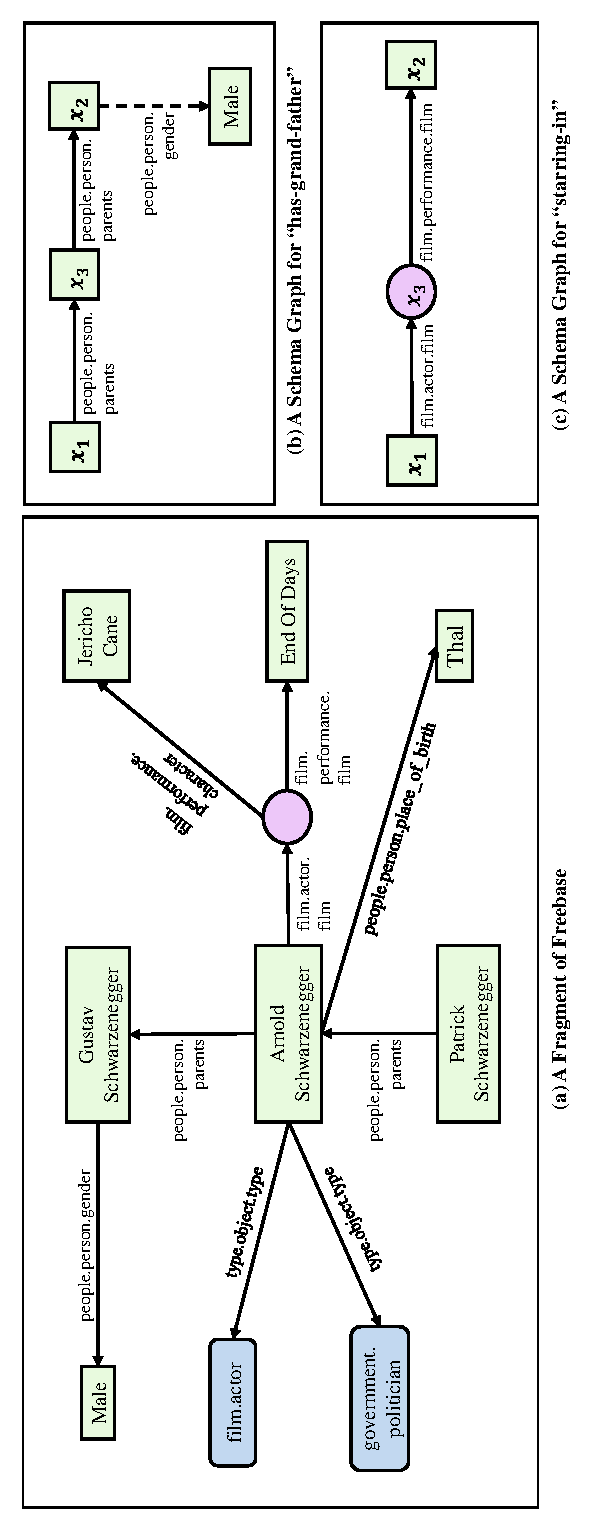
\epsfig{file=fb-schema.eps, width=0.95\columnwidth}
\centering
\scalebox{0.5}{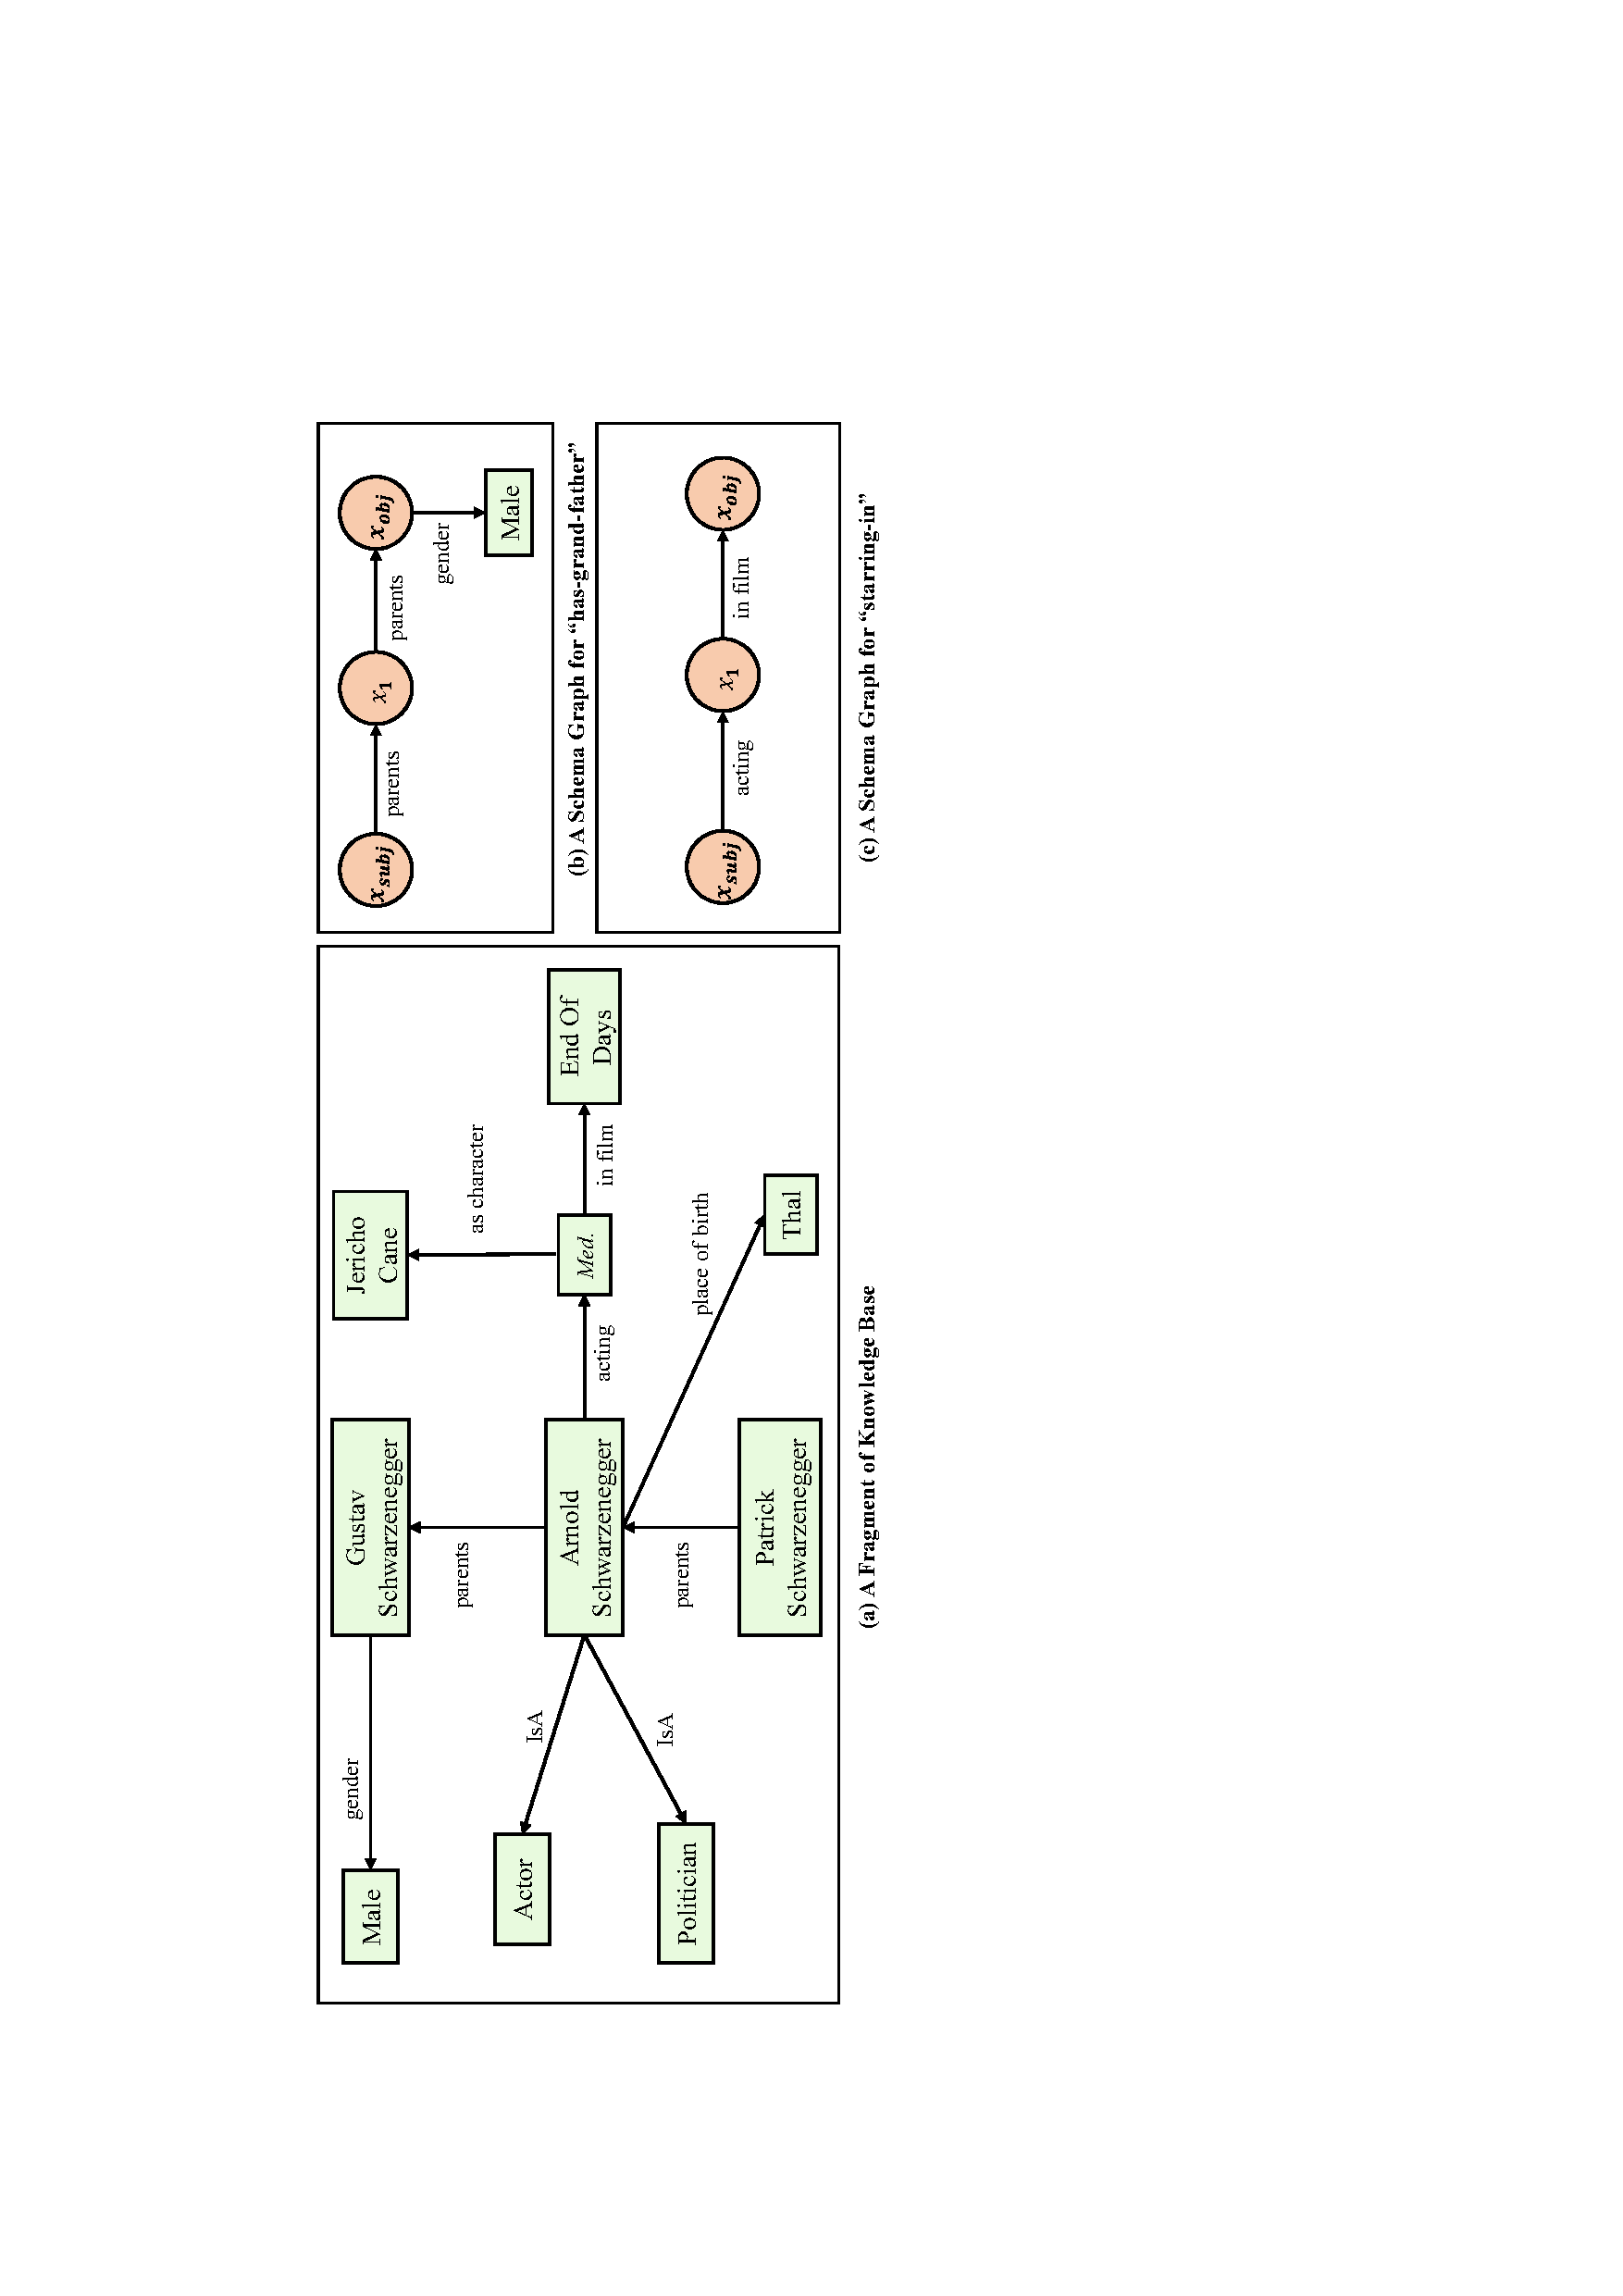
\includegraphics[angle=270]{kb-schema-crop.eps}}
\label{fig:kb-schema}
\caption{An example fragment of knowledge base and schema graphs.}
\end{figure*}


Though millions of facts are stored in such knowledge bases, 
they still face two key challenges.
% can not be perfectly used
First, the knowledge base is far from being complete, which gives rise to
an open research problem called knowledge base completion (KBC).
The goal of KBC is to populate predicates in a KB with new facts,
where both arguments of these new fact already exist in the knowledge base
as entities~\cite{gardner2015efficient,lao2010relational,lao2011random}.
Second, there are semantic gaps between KB predicates and 
natural language relations.
For example, Freebase doesn't have a precise predicate for 
``has grandfather'' relation, 
but instead has \textit{parent} and \textit{gender} predicates.

%One natural research question is,
%is it possible to enrich the facts in an incomplete knowledge base by
%integrating massive relation instances discovered from Open IE
%\cite{gardner2015efficient,lao2010relational,lao2011random}.
%That is, given a triple (``Madelyn Dunham'', ``grandfather of'',
%``Barack Obama'') extracted from open domain text,
%if both entities already exist in the knowledge
%base as distinct nodes, but not yet connected, can we connect them
%using existing predicates?
%%This task is also known as knowledge base completion (KBC).
%Another related question is, can we translate a natural language
%query such as ``Who is the grandfather of Patrick Schwarzenegger?''
%into a structured query to the knowledge base, using,
%for example, SPARQL.
%This question is relevant to automatic question answering
%\cite{berant2013semantic,berant2014semantic,yao2014information,zou2014natural},
%a major challenge in natural language processing.

These two challenges together form our research question:
given a relation and a set of its instances discovered by Open IE, 
is it possible to add a corresponding predicate into KB, 
and populate this predicate based on existing knowledge?
%Answer to the question: represent new relation by 
%existing structure knowledge rep.
The answer to the question lies in the ability to ``paraphrase''
a relation expressed in natural language patterns into some structured
knowledge representation.
As mentioned above, the predicates \textit{parent} and \textit{gender} 
may jointly represent the semantics of ``has grandfather'' 
(see \figref{fig:kb-schema}(b)).

%TODO: \KQ{Compared with traditional KBC tasks ... }

%For example, Freebase doesn't have has-grand-father predicate,
%or even has-father predicate, but instead has the {\em parent}
%and {\em gender} predicates, which may jointly represent the semantics
%of has-grand-father (see \figref{fig:kb-schema}(b)).

%There are different ways to represent relations in a knowledge graph.
%Previous work 
%\cite{gardner2015efficient,lao2011random,zou2014natural,zhang2012ontological}
%proposed to represent a relation by a {\em path} of
%predicates connecting the two entities in a knowledge base.
%Each node along the path is a variable entity of the type compatible
%with the predicates on either side of it. Such a path is
%called a {\em skeleton}.
%%along with discriminative
%%features on the edges and the nodes along the path.
%%\KZ{For example ...}.
%The advantages of such representation are
%i) it is intuitive; ii) it can be translated into
%SPARQL queries straightforwardly and hence all existing RDF tools
%can be used; and iii) it is human readable and allows manual fine-tuning
%if necessary.
%However, one limitation is that a path of predicates may not
%be accurate enough to represent a {\em complex} relation.
%For example, ``has grandfather'' relation could
%be represented by {\em parent} + {\em parent} path in Freebase,
%but this brings in additional noise since grandmothers are also included.

The state-of-the-art methods for this relational learning
%TODO: suitable to call "relational learning"?
task can be categorized into two branches.
The first branch is based on embedding technique
\cite{bordes2013translating,wang2014knowledge,guo2016jointly,wang2016text}
\KQ{missing refs: HOLE, CPRA, AMIE+, and ``statistic schema induction'',
since somehow I can't visit google scholar (either using proxy or not)}
%(TransE, TransH, Hole, Guo), %Name + Citation
,
which learns a vector representation for every entity and predicate in 
the knowledge base, then models relationships between two entities 
as vector translations in the embedding space.
These methods are able to learn hidden semantics of a target relation. 
However, with large amounts of parameters, such embedding model 
requires massive amount of triple facts as training data.
Moreover, due to large time and memory requrements in the training step,
previous works only perform experiments on subsets of the knowledge base
\cite{bordes2013translating,guo2016jointly},
rather than the full version.

On the other hand, rule induction techniques leverage explicit rules
as semantic representations of a target relation
\cite{lao2010relational,lao2011random,gardner2015efficient}.
%(SFE, PRA, CPRA, AMIE+)
Each rule is a substructure in the knowledge base, used to
connect the subject and object entities of the relation.
One of the most intuitive structure is {\em path}: a sequence of predicates
linking the subject to the object.
An advantage of rule induction methods is that structured 
rules can be translated into SPARQL queries and 
hence all existing RDF tools can be applied.
Rules are easily interpretable and human readable, 
which allows manual fine-tuning
if necessary (for example, finding potential ambiguities in one relation).
Because there are many possible rules in a given knowledge base,
it's challenging to find the most effective rules.
%\KQ{Currently we don't talk about the others disadvantages of skeleton based method,
%since we will discuss the advantage of schemas in the later part of this section.}
%Another problem is that the selection of such features can be
%random and ad hoc.
%For example, {\em anyrel} is a feature that represents any predicate
%in the knowledge graph; the difference between the numerical values
%on two different nodes can be a feature as well. A more serious
%disadvantage is that such representation cannot be readily translated into
%SPARQL queries. Instead additional program code must be written to support
%queries, such as whether $e_1$ and $e_2$ has certain relation, or given
%$e_1$ and a relation, what is $e_2$. Finally, feature-based approach
%represents a relation by a bunch of weights, which are not human
%readable and are hard to explain.
In this paper, we propose to generalize the path structure
into a tree structure connecting not only the two target entities, but also
other constants and constraints around the path connecting the two. 
This tree structure is an abstraction of a set of all 
concrete sub-trees in the knowledge base having the same edge
structure.
%Another perhaps more natural representation of a type of relation
%in a knowledge graph is a subgraph structure. This subgraph
%is an abstraction of all the concrete subgraphs of the same shape
%that connects each individual pair of the entities in the knowledge graph.
%This subgraph connects constant entities as well as variables.
We call such a tree structure a {\em schema graph}, or {\em schema}
in short.  \figref{fig:kb-schema}(b) and (c) give two example of
such schema graphs, which are essentially views 
on the knowledge base, joining several primitive predicates together.
%For example, the has-grand-parent relation can be represented by
%the Freebase schema shown in \figref{fig:kb-schema}(b), while
%the starring-in relation can be represented in \figref{fig:kb-schema}(c).

Informally, the input of the paraphrasing task is a list of entity pairs
$(e_1, e_2)$ extracted by natural language relation pattern $r$,
%with its surface form,
and the output is a set of schema graphs with probabilities to measure
their ability to represent the relation $r$ in the knowledge base.
%The schema representation is formed in a tree structure, which
%consists of the predicate path connecting two entities directly,
%and constraint predicates at the branch of the path.
%Therefore, our paraphrasing task is the generalization of previous
%path-based work.
This generalization is important because complex relations that
require constraints constitute a non-trivial portion of all extracted
relations from open IE.
For example, by manual inspection, out of 2,500 most popular 
relation patterns in PATTY dataset,  13\% of the relation
instances and 7.5\% \KQ{18\% in our experiment} of relation patterns
are actually complex (i.e., require more than a simple path to represent).

%The challenges for inferring a schema representation are two-fold.
There are three main challenges for inferring a schema representation.
First, there are many possible schema graphs that potentially
connect a pair of entities, and a brute force search over all schemas
is intractable.
Second, because the learning process is data driven, i.e.,
only relation instances and not schemas are available for training,
the learning model needs to trade off between general, high recall but
low precision schemas (e.g., parents + parents) versus specific, high
precision but low recall schemas (e.g., parents + parents + gender=male).
Third, with only positive training data which are entity pairs, 
the learning task is difficult.
As a circumvention, one can use the close world assumption to automatically
generate negative instances. But due to data incompleteness of KB,
potential false negatives may cause problem.
%In general, simpler schemas tend to be more general in meaning,
%whereas more complex schemas are more specific in meaning.
%A schema that is too general is less expressive and less informative,
%while a schema that is too specific may not be able to cover all
%the entity pairs.
This paper addresses these challenges and makes the following contributions.

%We define the notion \textbf{simple schema}, if the schema graph cotains \textit{only}
%a path of predicates connecting entities from $e_1$ to $e_2$ in the knowledge base.
%To this end, state-of-the-art systems have been proposed for solving this task.
%

%2. what's knowledge base try to do
%Structured knowledge base (KB) is a graph based taxonomy containing real world
%entities,  types,  binary predicates between entities and ``IsA'' relations
%between entities and types.
%(Machine readable, containing millions / billions of facts)

%Structured KBs such as WordNet \cite{miller1995wordnet},
%Yago \cite{suchanek2007WWW} and Freebase \cite{bollacker2008freebase} are widely used in information extraction
%and semantic learning tasks. In order to make relation schemas understood by human, we leverage types
%in the KB as the output of relation schemas.

%3. what to do is to extract schema
%The paraphrasing task is to map a natural language relation into structured
%canonical forms in KB, which is understood by both machine and human.
%
%We call the representation as \textit{relation schema} throughout this paper.
%
%\KQ{how to give a clear impression on schema}
%%\cite{bollacker2008freebase}
%%%Figure show schema on FB as the first impression (mention FB's size here)
%informal
%One can see that a relational schema is a template of many subgraphs
%with the concrete structure in the knowledge base.
%The goal of this paper is to enable effective and efficient translation
%process, which we call ``paraphrasing.''


%add. why we need to schema
%Paraphrasing is a open task, since the structured schema is an important knowledge
%used in many down-stream applications, such as question answering, text entailment
%and short text similarity querying.
%(Arguing)

%1. why we need paraphrasing

%2. what's the advantage of schema
% SPARQL query
% user intent query (check view synthesis paper)
%Paraphrasing is a fundamental task in natural language processing and understanding,
%especially in the system of question answering ,
%and knowledge base completion.
%In these tasks, the relation coming from input sentence (or question) is transformed
%into semantic structure in the knowledge base, and the overall accuracy is largely
%determined by the quality of the structural representation.
%
%
%There are three main advantages for our schema based model.
%First, each schema is an independent structure that represents the target relation.
%Feature weights produced by discriminative model can tell us which schemas are more
%suitable for the relation, while a single feature snippet is less expressive.
%Second, the schema is a subgraph of a semantic knowledge base.
%Our system can easily transform a schema into a SPARQL query due to the widely used RDF model
%in semantic knowledge bases. Therefore, an end-user can query RDF to retrive instances
%or a natural language relation, even though they don't know how to write a SPARQL query.
%Third, the schema is human-readable. Interactive online QA systems can display schemas and
%allow end-users to adjust them, leading to a better user experience.
%
%

%4. claim the gap between kb and nl on description
%Recap the semantic gap between relations and knowledge base predicates that we mentioned
%Yet some knowledge base is lack of predicates, however, the gap couldn't be removed,
%even for Freebase containing thousands of binary predicates.
%%5. simple exmple & chain example (mediator)
%%6. branching example
%%a) place_of_birth v.s. <people, was born in, place>
%%b) mediator: film.actor.film --> film.performance.film   v.s.   "starring in"
%%c) branching: female spouse v.s. "wife of"
%The predicate name ``place\_of\_birth'' in \figref{fig:fb-schema} (a) shows the difference,
%compared with relation words ``was born in'';
%\figref{fig:fb-schema} (b) brings the gap to structural level, where the schema shows a
%complex ``parent + parent + male'' style, even ``grandfather'' relation is so common in
%the real world; Meanwhile, \figref{fig:fb-schema} (c) show that the schema must include
%a intermediate node (used to maintain the ternary relation ``actor plays a character in a film'').
%These varieties make the paraphrase task challenging.
%
%%traditional method & limits
%%0. informally, composite relation
%%(Lei Zou) (EMNLP 2011) (AAAI 2012) (Tran 2009) (EMNLP 2015)
%For the part of feature based supervised systems, the first branch is graph-walk based
%\cite{lao2010relational,lao2011random}, a candidate schema is drawn from the predicate path
%between some entity pairs, and the probabilistic distribution of random walking from $e_1$
%to $e_2$ in KB on the schema is used as a feature to train the importance of each path.
%The second branch is logic based \cite{zhang2012ontological}, where the system uses hand
%crafted soft rules to mine various features that leads to good relation schemas.
%Since soft rules are fixed and independent of relations, the dimension of feature space
%is limited.
%
%Besides, unsupervised models are also used. Zou et al. \cite{zou2014natural}
%followed the idea of TF-IDF score \cite{blabla} to calculate the best schema with respect to a
%speicifc relation. While different input relations could have overlap meaning, this situation
%causes a lower score of schemas representing the overlapping part.
%
%In addition, among all different paraphrasing solvers, the process of candidate schema
%searching could always be a big challenge. All systems discussed above only generate
%simple schemas (predicate paths), which is also a limitation for searching more
%specific and meaningful schemas.
%
% our approach
%1. IMPORTANT data-driven

%We present a distant-supervised learning approach to solve the
%paraphrasing problem, with the following contributions:
\begin{itemize}
\itemsep0em
\item We define schemas as a generalized representation of natural language
relations in knowledge base (\secref{sec:problem});
\item %Due to the prohibitive space of possible schemas,
We present an effective local search based heuristic to generate a set of
candidate schemas (\secref{sec:candgen});
\item We propose a data-driven approach to model the schema inference
problem as a querying task, and thus compute the probability of a schema
given a natural language relation and its instances
without explicitly generating negative data (\secref{sec:schema});
\item The framework significantly outperforms 
previous best approaches on knowledge base completion task,
the example results show that our schema paraphrasing model
is able to discover concrete and precise semantics (\secref{sec:eval}).
%and question answering. Furthermore, our schema representation is
%on par with the popular word embedding model in computing relation similarity (\secref{sec:eval}).
\end{itemize}
